% Template of basic phisics experiment 基于 article template, 在此基础上做修改
% 设定文章编码类型, 正文字号为五号则 zihao=5, 正文字号为小四则 zihao=-4
\documentclass[zihao=5, UTF8]{article}		


% 自定义宏定义
\def\N{\mathbb{N}}
\def\F{\mathbb{F}}
\def\Z{\mathbb{Z}}
\def\Q{\mathbb{Q}}
\def\R{\mathbb{R}}
\def\C{\mathbb{C}}
\def\T{\mathbb{T}}
\def\S{\mathbb{S}}
\def\A{\mathbb{A}}
\def\I{\mathscr{I}}
\def\d{\mathrm{d}}
\def\p{\partial}


% 物理实验报告所需的其它宏包
\usepackage{ulem}   % \uline 下划线支持

% 导入基本宏包
\usepackage[UTF8]{ctex}     % 设置文档为中文语言
\usepackage[colorlinks, linkcolor=blue, anchorcolor=blue, citecolor=blue, urlcolor=blue]{hyperref}  % 宏包：自动生成超链接 (此宏包与标题中的数学环境冲突)
% \usepackage{docmute}    % 宏包：子文件导入时自动去除导言区, 用于主/子文件的写作方式, \include{./51单片机笔记}即可. 注：启用此宏包会导致.tex文件capacity受限. 
\usepackage{amsmath}    % 宏包：数学公式
\usepackage{mathrsfs}   % 宏包：提供更多数学符号
\usepackage{amssymb}    % 宏包：提供更多数学符号
\usepackage{pifont}     % 宏包：提供了特殊符号和字体
\usepackage{extarrows}  % 宏包：更多箭头符号
\usepackage{multirow}

% 列表环境设置
\usepackage{enumitem}   % 宏包：列表环境设置
    \setlist[enumerate]{itemsep=0pt, parsep=0pt, topsep=0pt, partopsep=0pt, leftmargin=3.5em} 
    \setlist[itemize]{itemsep=0pt, parsep=0pt, topsep=0pt, partopsep=0pt, leftmargin=3.5em}
    \newlist{circledenum}{enumerate}{1} % 创建一个新的枚举环境  
    \setlist[circledenum,1]{  
        label=\protect\circled{\arabic*}, % 使用 \arabic* 来获取当前枚举计数器的值, 并用 \circled 包装它  
        ref=\arabic*, % 如果需要引用列表项, 这将决定引用格式（这里仍然使用数字）
        itemsep=0pt, parsep=0pt, topsep=0pt, partopsep=0pt, leftmargin=3.5em
    }  
% 文章页面 margin 设置
\usepackage[a4paper]{geometry}  % 宏包：文章页面 margin 设置
    \geometry{top=0.75in}
    \geometry{bottom=0.75in}
    \geometry{left=0.75in}
    \geometry{right=0.75in}   % 设置上下左右页边距
    \geometry{marginparwidth=1.75cm}    % 设置边注距离（注释、标记等）

% 自定义数学环境
\usepackage{amsthm} % 宏包：数学环境配置
% theorem-line 环境自定义
    \newtheoremstyle{MyLineTheoremStyle}% <name>
        {11pt}% <space above>
        {11pt}% <space below>
        {}% <body font> 使用默认正文字体
        {}% <indent amount>
        {\bfseries}% <theorem head font> 设置标题项为加粗
        {：}% <punctuation after theorem head>
        {.5em}% <space after theorem head>
        {\textbf{#1}\thmnumber{#2}\ \ (\,\textbf{#3}\,)}% 设置标题内容顺序
    \theoremstyle{MyLineTheoremStyle} % 应用自定义的定理样式
    \newtheorem{LineTheorem}{Theorem.\,}
% theorem-block 环境自定义
    \newtheoremstyle{MyBlockTheoremStyle}% <name>
        {11pt}% <space above>
        {11pt}% <space below>
        {}% <body font> 使用默认正文字体
        {}% <indent amount>
        {\bfseries}% <theorem head font> 设置标题项为加粗
        {：\\ \indent}% <punctuation after theorem head>
        {.5em}% <space after theorem head>
        {\textbf{#1}\thmnumber{#2}\ \ (\,\textbf{#3}\,)}% 设置标题内容顺序
    \theoremstyle{MyBlockTheoremStyle} % 应用自定义的定理样式
    \newtheorem{BlockTheorem}[LineTheorem]{Theorem.\,} % 使用 LineTheorem 的计数器
% definition 环境自定义
    \newtheoremstyle{MySubsubsectionStyle}% <name>
        {11pt}% <space above>
        {11pt}% <space below>
        {}% <body font> 使用默认正文字体
        {}% <indent amount>
        {\bfseries}% <theorem head font> 设置标题项为加粗
        {：\\ \indent}% <punctuation after theorem head>
        {0pt}% <space after theorem head>
        {\textbf{#3}}% 设置标题内容顺序
    \theoremstyle{MySubsubsectionStyle} % 应用自定义的定理样式
    \newtheorem{definition}{}


% 有色文本框及其设置
\usepackage[dvipsnames,svgnames]{xcolor}    %设置插入的文本框颜色
\usepackage[strict]{changepage}     % 提供一个 adjustwidth 环境
\usepackage{framed}     % 实现方框效果
    \definecolor{graybox_color}{rgb}{0.95,0.95,0.96} % 文本框颜色. 修改此行中的 rgb 数值即可改变方框纹颜色, 具体颜色的rgb数值可以在网站https://colordrop.io/ 中获得. （截止目前的尝试还没有成功过, 感觉单位不一样）（找到喜欢的颜色, 点击下方的小眼睛, 找到rgb值, 复制修改即可）
    \newenvironment{graybox}{%
    \def\FrameCommand{%
    \hspace{1pt}%
    {\color{gray}\small \vrule width 2pt}%
    {\color{graybox_color}\vrule width 4pt}%
    \colorbox{graybox_color}%
    }%
    \MakeFramed{\advance\hsize-\width\FrameRestore}%
    \noindent\hspace{-4.55pt}% disable indenting first paragraph
    \begin{adjustwidth}{}{7pt}%
    \vspace{2pt}\vspace{2pt}%
    }
    {%
    \vspace{2pt}\end{adjustwidth}\endMakeFramed%
    }

% 各级标题自定义设置
\usepackage{titlesec}   
    % section标题自定义设置 
    \titleformat{\section}[hang]{\normalfont\huge\bfseries\centering}{第\,\thesection\,部分}{20pt}{}
    % subsection标题自定义设置 
    \titleformat{\subsection}[hang]{\normalfont\Large\bfseries}{\,\thesubsection\,}{8pt}{}
    % subsubsection标题自定义设置
    \titleformat{\subsubsection}[hang]{\normalfont\large\bfseries}{\,\thesubsubsection\,}{6pt}{}

% 外源代码插入设置
\usepackage{matlab-prettifier}
    \lstset{
        style=Matlab-editor,  % 继承matlab代码颜色等
    }
\usepackage[most]{tcolorbox} % 引入tcolorbox包 
\usepackage{listings} % 引入listings包
    \tcbuselibrary{listings, skins, breakable}
    \lstdefinestyle{matlabstyle}{
        language=Matlab,
        basicstyle=\small,
        breakatwhitespace=false,
        breaklines=true,
        captionpos=b,
        keepspaces=true,
        numbers=left,
        numbersep=15pt,
        showspaces=false,
        showstringspaces=false,
        showtabs=false,
        tabsize=2
    }
    \newtcblisting{matlablisting}{
        arc=0pt,
        top=0pt,
        bottom=0pt,
        left=1mm,
        listing only,
        listing style=matlabstyle,
        breakable,
        colback=white   % 选一个合适的颜色
    }

% table 支持
\usepackage{booktabs}   % 宏包：三线表
\usepackage{tabularray} % 宏包：表格排版
\usepackage{longtable}  % 宏包：长表格

% figure 设置
\usepackage{graphicx}  % 支持 jpg, png, eps, pdf 图片 
\usepackage{svg}       % 支持 svg 图片
    \svgsetup{
        % 指向 inkscape.exe 的路径
        inkscapeexe = C:/aa_MySame/inkscape/bin/inkscape.exe, 
        % 一定程度上修复导入后图片文字溢出几何图形的问题
        inkscapelatex = false                 
    }


% 图表进阶设置
\usepackage{float}     % 图表位置浮动设置 
\usepackage{caption}    % 图注、表注
    \captionsetup[figure]{name=图}  
    \captionsetup[table]{name=表}
    \captionsetup{labelfont=bf, font=small}

% 文章默认字体设置
    \usepackage{fontspec}   % 宏包：字体设置
        \setmainfont{SimSun}[
            BoldFont = SimHei, % 设置粗体字为黑体
            ItalicFont = KaiTi, % 设置斜体字为楷体
            BoldItalicFont = KaiTi % 设置粗斜体字为楷体
        ] 
        %\setCJKmainfont[AutoFakeBold=3]{SimSun} % 设置加粗字体为 SimSun 族, AutoFakeBold 可以调整字体粗细
        \setmainfont{Times New Roman} % 设置英文字体为Times New Roman


% 其它设置
    % equation 公式编号设置
        \makeatletter  
        \renewcommand{\theequation}{\thesection.\arabic{equation}}  
        \makeatother
    % 脚注设置
        \renewcommand\thefootnote{\ding{\numexpr171+\value{footnote}}}
    % 参考文献引用设置
        \bibliographystyle{unsrt}   % 设置参考文献引用格式为unsrt
        \newcommand{\upcite}[1]{\textsuperscript{\cite{#1}}}     % 自定义上角标式引用
    % 文章序言设置
        \newcommand{\cnabstractname}{序言}
        \newenvironment{cnabstract}{%
            \par\Large
            \noindent\mbox{}\hfill{\bfseries \cnabstractname}\hfill\mbox{}\par
            \vskip 2.5ex
            }{\par\vskip 2.5ex}


% 页眉页脚设置
\usepackage{fancyhdr}   %宏包：页眉页脚设置
    \pagestyle{fancy}
    \fancyhf{}
    \cfoot{\thepage}
    \renewcommand\headrulewidth{1pt}
    \renewcommand\footrulewidth{0pt}
    \rhead{\bfseries 分组序号: 3-04-1}    
    \chead{《基础物理实验》实验报告,\ 潘天麟\ 2023K8009908023}
    \lhead{2024.10.30}

\usepackage{pdfpages}

% 开始编辑文章

\begin{document}
\noindent\begin{flushright}
    \zihao{2}{分组序号: 3-04-1}
\end{flushright}

\setCJKfamilyfont{boldsong}[AutoFakeBold = {2.17}]{SimSun}
\newcommand*{\boldsong}{\CJKfamily{boldsong}}


\begin{center}\large
    \noindent{\Huge\bfseries\boldsong《基础物理实验》实验报告 }
    \\\vspace{0.4cm}
    \noindent\textit{
        \textbf{\boldsong 实验名称：}\uline{\hspace{2.3cm} 杨氏模量\hspace{2.3cm}}\hspace{0.4cm} 
        指导教师：\uline{\hspace{1.5cm}任意\hspace{1.5cm}}}
    \\\vspace{0.1cm}
    \noindent\textit{
        姓名：\uline{\,\,潘天麟\,\,}\hspace{0.2cm}
        学号：\uline{\,\,{\upshape 2023K8009908023}\,\,}\hspace{0.2cm}
        专业：\uline{\,\,人工智能\,\,}\hspace{0.2cm}
        班级：\uline{\,\,\upshape{2313}\,\,}\,组号：\uline{\,\,\upshape{3-04-1}\,\,}}
    \\\vspace{0.1cm}
    \noindent\textit{
        实验日期：\uline{\,\,{\upshape 2024.10.30}\,\,}\hspace{0.2cm}
        实验地点：\uline{\,\,\,教学楼{\upshape710}\,\,\,}\hspace{0.2cm}
        是否调课/补课：\uline{\hspace{1.3cm}}\hspace{0.2cm}
        成绩：\uline{\hspace{2cm}}}
\end{center}
% \vspace{-0.2cm}
\noindent\rule{\textwidth}{0.1em}   % 分割线
\section{拉伸法测定金属的杨氏模量}
\subsection{实验目的}
\begin{enumerate}
    \item 理解各种静态方法测杨氏模量及其测量微小位移方法的原理及优缺点，了解动态法测杨氏模量的原理
    \item 学会读数望远镜、读数显微镜的调节
    \item 学习用逐差法、作图法和最小二乘法处理数据
    \item 学会计算各物理量的不确定度，并用不确定度正确表达实验结果
\end{enumerate}
\subsection{实验仪器}
\subsubsection{CCD 杨氏弹性模量测量仪}
\begin{enumerate}
    \item 采用分化板 + CCD 测量显微镜系统 + 彩色液晶监视器方案；
    \item 立柱：不锈钢双柱高约 85 cm；
    \item 金属丝：钼丝或钢丝，长约 60 cm，悬挂位置及长度可调节；
    \item 监视器：彩色液晶监视器；
    \item 分化板：刻度范围 4 mm, 分度值 0.05 mm，设有限位槽，可防止来回摆动，采用 LED 照明；
    \item CCD 测量显微镜系统：放大倍率 60 倍，内含电子刻度线，可二维调节，可卸下用于其他微位移测量场合，采用高级面阵 CCD，信噪比 $\geq 52 \text{ dB}$，分辨率 480 TVL，视频输出幅度：1.0 VP-P/75Ω；
    \item 砝码组：10 个砝码，200 克 8 个及 100 克 2 个；
    \item 底座沉稳，可进行水平调节，设有储藏格可贮存砝码组；
    \item 测量相对不确定度：$< 5\%$；
    \item 读数显微镜：放大倍数 15×；
    \item 测量架：测量范围：0—4 mm；
    \item 下夹头：含有数字分划板，分划板数值：0.05 mm；
    \item CCD：12V 电源 3；
    \item 显视器：彩色液晶监视器（纯正品）；
    \item 钼丝：$L = 1000 \, \Phi 0.18$；
    \item 不锈钢丝：$L = 1000 \, \Phi 0.30$；
    \item 光学平台：精密铸造，台面含磁不锈钢板。尺寸：$405 \, \text{mm} \times 308 \, \text{mm} \times 39 \, \text{mm}$；
    \item 二维磁力滑座：含有横向纵向及垂直精密移动装置；
    \item 镀铬钢制砝码：重量：250 g/个 数量：8 个；
    \item 水准器：$\Phi 40 \, \text{mm}$；
\end{enumerate}
\subsubsection{螺旋测微器}
量程0-25mm，分度值0.01mm
\subsubsection{钢卷尺}
量程3m，最小分度值1mm
\subsection{实验原理}
当金属被拉伸时，正应力与线应变在弹性范围内成正比，也就是
\begin{equation}
\frac{F}{S} = Y \frac{\Delta L}{L}
\end{equation}
其中$Y$被称为杨氏模量。实验中将金属丝上端固定，下端添加砝码产生力$F$，用螺旋测微器测出金属丝的直径后根据$S = \pi d^{2}$得到横截面积。我们可以在CCD显示屏上读出$ \Delta L $，并用钢卷尺读出金属丝长度$L$，然后根据上述公式即可算出金属丝的杨氏模量。

当天平上增加了质量为$M$的砝码后，力$F$增加了$Mg$，插丝板通过显微镜显示在分划板上，再通过目镜放大后即可通过肉眼观察到金属丝长度的变化量，也就是$\Delta L$。
\subsection{实验内容}
\subsubsection{仪器调节}
调节支架：底座用螺旋底角调平，叉丝组分划板正对CCD摄像头。调节下横梁高度，保证叉丝组放置在下横梁的槽内。

调节CCD摄像机：将CCD摄像头放入固定座内，将CCD摄像头与分划板放置在同一水平面上，前后调节CCD摄像头观察监视器，直到可以观察到清晰的像，若分划板刻度尺不在监视器的中心，则微调CCD摄像头位置使像处于中心位置。

\subsubsection{测量}
\begin{enumerate}
    \item 在测量钼丝杨氏模量前，先放1块250 g的砝码把钼丝拉直，保证分划板卡在下横梁的槽内，这样可以避免在拉直过程中分划板旋转。
    \item 记下待测细丝下的砝码盘未加砝码时屏幕上显示的毫米尺在横线上的读数 $l_0=0$，以后在砝码盘上每增加一个 $M=250 \, \text{g}$ 的砝码，记下相应的叉丝读数 $l_i \, (i=1,2,\cdots,8)$。然后逐一减掉砝码，再从屏上读取 $l_i' \, (i=1,2,\cdots,7)$。
    \item 取同一负荷下叉丝读数的平均值 $\overline{l_i}$，用逐差法求出钼丝荷重增减4个砝码时光标的平均偏移量 $\Delta L$。
    \item 用钢卷尺测量上、下夹头间的钼丝长度 $L$。
    \item 用螺旋测微器测量钼丝直径 $d$，由于钼丝直径可能不均匀，按工程要求应在上、中、下各部进行测量。每位置在相互垂直的方向各测一次。
    \item 将前述原理公式分解整理即得：
    \begin{equation}
        Y = \frac{4MgL}{\pi d^2 \Delta L}
    \end{equation}
        钼丝的杨氏模量 $Y$ 约为 $2.3 \times 10^{11} \, \text{N} \cdot \text{m}^{-2}$。
\end{enumerate}
\subsection{实验数据}
\begin{itemize}
    \item 钼丝长度 $L = 796.5$mm, 卷尺仪器误差 $e = \pm 2.0$mm
    \item 钼丝直径
        \begin{table}[H]
            \centering
            \begin{tabular}{|cccccccc|}
                \hline
                测量次数 & 1 & 2 & 3 & 4 & 5 & 6 & 平均值 $\bar{d}$ \\
                \hline
                d/mm & 0.336 & 0.358 & 0.369 & 0.337 & 0.342 & 0.351 & 0.349 \\
                \hline
            \end{tabular}
            \caption{钼丝直径测量结果}
        \end{table}
    \item 监视器示数
        
        初始示数$l_0 = 0.10$mm, 千分尺仪器误差 $e = \pm 0.005$mm
        \begin{table}[h!]
            \centering
            \begin{tabular}{|c|c|c|c|c|c|c|c|c|c|}
                \hline
                \multirow{2}{*}{\shortstack{序号 \\ $i$}} & \multirow{2}{*}{\shortstack{砝码质量 \\ $M$/g}} & \multicolumn{3}{c|}{叉丝读数/mm} & \multirow{2}{*}{\shortstack{$l_i M_i$ \\ /(mm $\cdot$ g)}} & \multirow{2}{*}{\shortstack{示数差值 \\ $\Delta l_i = \bar{l}_{i+4} - \bar{l}_i$}} & \multirow{2}{*}{\shortstack{不确定度 \\ $\Delta(\Delta l)$}} \\
                \cline{3-5}
                & & 加载 $l_i$/mm & 卸载 $l'_i$/mm & 平均值 $\bar{l}_i$/mm & & & \\
                \hline
                1 & 250 & 0.35 & 0.35 & 0.35 & 87.5 & 0.73 & \\
                \cline{1-7}
                2 & 500 & 0.57 & 0.54  & 0.56 & 280 & 0.69 & \\
                \cline{1-7}
                3 & 750 & 0.75 & 0.73 & 0.74 & 555 & 0.66 & \\
                \cline{1-7}
                4 & 1000 & 0.92 & 0.94 & 0.93 & 930 & 0.59 & \multirow{2}{*}{0.01} \\
                \cline{1-7}
                5 & 1250 & 1.08 & 1.08 & 1.08 & 1350 & & \\
                \cline{1-7}
                6 & 1500 & 1.25 & 1.25 & 1.25 & 1875 & & \\
                \cline{1-7}
                7 & 1750 & 1.37 & 1.42 & 1.40 & 2450 & & \\
                \cline{1-7}
                8 & 2000 & 1.52 & 1.52 & 1.52 & 3040& & \\
                \hline
                {$\overline{M}$} & 1125 & & {$\bar{\bar{l}}$} & 0.98 & & & \\
                \cline{1-2} \cline{4-5}
                $\Sigma M$ & 9000 & & $\Sigma \bar{l}$ & 7.83 & & & \\
                \hline
            \end{tabular}
            \caption{叉丝读数数据记录表}
        \end{table}
\end{itemize}
\subsection{数据处理}
\subsubsection{计算钼丝长度}
利用卷尺对加上250 g砝码后钼丝的长度$L$进行单次测量，测量结果为$L = 796.5 \, \text{mm}$。由于测量次数为6，所以A类不确定度
\[
u_A (L) = \sqrt{\frac{\sum_{i=1}^{6} (L_i - \bar{L})^2}{6(6-1)}} = \sqrt{\frac{1.0^2 + 0.9^2 + 1.1^2 + 0.1^2 + 0.5^2 + 0.9^2}{30}} = \sqrt{0.14} \, \text{mm}
\]
由于卷尺的允差$e = \pm2$mm，所以B类不确定度为
\[
u_B (L) = \frac{e}{\sqrt{3}} = \frac{2}{\sqrt{3}} \, \text{mm}
\]
所以测量钼丝长度的不确定度 $u(L)$ 为
\[
u(L) = \sqrt{u_A (L)^2 + u_B (L)^2} = \sqrt{\frac{2^2}{3} + 0.14} = 1.2 \, \text{mm}
\]
其相对不确定度为
\[
\frac{u(L)}{L} = \frac{1.2}{796.5} \times 100\% = 0.15\%
\]
钼丝的长度为
\[
L = (796.5 \pm 1.2) \, \text{mm}
\]

\subsubsection{计算钼丝直径}
根据表1中数据计算可得，测量6次直径带来的A类不确定度为
\[
u_A (d) = \sqrt{\frac{\sum_{i=1}^{6} (d_i - \bar{d})^2}{5 \times 6}} = \sqrt{\frac{0.01^2 + 0.01^2 + 0.02^2 + 0.01^2 + 0^2 + 0^2}{5 \times 6}} = 0.005 \, \text{mm}
\]
由于螺旋测微器的允差为 $e = 0.005$ mm，所以B类不确定度为
\[
u_B (d) = \frac{e}{\sqrt{3}} = \frac{0.005}{\sqrt{3}}
\]
所以测量钼丝直径的合成不确定度为
\[
u(d) = \sqrt{u_A (d)^2 + u_B (d)^2} = \sqrt{0.005^2 + \frac{0.005^2}{3}} = 0.006 \, \text{mm}
\]
其相对不确定度为
\[
\frac{u(d)}{\bar{d}} = \frac{0.006}{0.349} \times 100\% = 1.7\%
\]
钼丝的直径为
\[
d = (0.349 \pm 0.006) \, \text{mm}
\]

\subsubsection{计算加减砝码后钼丝长度变化}
由表2中数据可知，钼丝的长度变化平均值为
\[
\bar{\Delta l} = \frac{1}{4} (0.73 + 0.69 + 0.66 + 0.59) = 0.67 \, \text{mm}
\]
由不确定度的传递公式
\[
\Delta(\bar{\Delta l}) = u(\bar{\Delta l}) = \frac{1}{4} \sqrt{u(\Delta l_1)^2 + u(\Delta l_2)^2 + u(\Delta l_3)^2 + u(\Delta l_4)^2}
\]
其中
\[
\begin{aligned}
&u(\Delta l_i) = \sqrt{u(l_{i+4})^2 + u(l_i)^2},
&u(l_i) = \sqrt{u_A (l_i)^2 + u_B (l_i)^2} \\
&u_A (l_i) = \sqrt{\frac{(l_i - \bar{l_i})^2 + (l_i' - \bar{l_i})^2}{2}} ,
&u_B (l_i) = \frac{e}{\sqrt{3}} = \frac{0.005}{\sqrt{3}} \, \text{mm}
\end{aligned}
\]
再根据表2中数据计算可得
\begin{table}[H]
    \centering
    \begin{tabular}{|c|c|c|c|c|c|c|c|c|}
        \hline
        $i$ & 1 & 2 & 3 & 4 & 5 & 6 & 7 & 8 \\
        \hline
        $u_A(l_i)$/mm  & 0.00 & 0.02 & 0.01 & 0.01 & 0.00 & 0.00 & 0.02 & 0.00\\
        \hline
        $u(l_i)$/mm  & 0.00 & 0.02 & 0.01 & 0.01 & 0.00 & 0.00 & 0.02 & 0.00\\
        \hline
        $u(\Delta l_i)$/mm  & 0.00 & 0.02 & 0.03 & 0.01 &  &  &  & \\
        \hline
    \end{tabular}
    \caption{钼丝长度变化量不确定数据计算}
\end{table}
因此
\[
\Delta(\overline{\Delta l}) ) = \frac{1}{4} \sqrt{0.00^2 + 0.03^2 + 0.03^2 + 0.01^2} = 0.01 \, \text{mm}.
\]
其相对不确定度为：
\[
\frac{u(\Delta l)}{(\Delta l) ̅} = \frac{0.01}{0.67} \times 100\% = 1.5\%.
\]
钼丝的长度变化为：
\[
\Delta l = (0.67 \pm 0.01) \, \text{mm}.
\]
\subsubsection{用逐差法处理杨氏模量}
我们直接由公式计算：
\[
Y = \frac{4 \Delta M g L}{\pi d^2 \Delta l} = \frac{4 \times (1000 \times 10^{-3}) \times 9.81 \times (796.5 \times 10^{-3})}{\pi \times (0.349 \times 10^{-3})^2 \times (0.67 \times 10^{-3})} = 1.22 \times 10^{11} \, \text{N} \cdot \text{m}^{-2}.
\]
由不确定度的传递公式：
\[
\frac{u(Y)}{Y} = \sqrt{\left(\frac{u(L)}{L}\right)^2 + \left(\frac{u((\Delta l) ̅)}{(\Delta l) ̅}\right)^2 + \left(2 \frac{u(d)}{d}\right)^2} = \sqrt{\left(\frac{1.2}{796.5}\right)^2 + \left(\frac{0.01}{0.67}\right)^2 + \left(2 \times \frac{0.006}{0.349}\right)^2} = 0.04.
\]
因此杨氏模量的不确定度为：
\[
u(Y) = 0.04 \times 1.22 \times 10^{11} = 0.05 \times 10^{11} \, \text{N} \cdot \text{m}^{-2}.
\]
因此：
\[
Y = (1.22 \pm 0.05) \times 10^{11} \, \text{N} \cdot \text{m}^{-2}.
\]
相对误差为：
\[
E_r (Y) = \frac{|Y - Y_0|}{Y_0} \times 100\% = \frac{(2.3 - 1.22)}{2.3} \times 100\% = 46.96\%.
\]

\subsubsection{用最小二乘法处理杨氏模量}
已知
\[
l_i = \frac{L}{Y} \cdot \frac{m_i g}{S} + l_0 - l = k m_i + b
\]
其中
\[
k = \frac{L g}{Y S} = \frac{4gL}{\pi Y d^2}
\]
以 $m_i$ 为横坐标，以 $\bar{l_i}$ 为纵坐标，进行最小二乘法拟合可得
\[
k = \frac{\sum M_i \bar{l_i} - \frac{(\sum M_i)(\sum \bar{l_i})}{n}}{\sum M_i^2 - \frac{(\sum M_i)^2}{n}} = \frac{10556 - \frac{9000 \times 7.83}{8}}{1.28 \times 10^7 - 1.01 \times 10^7} = 6.47 \times 10^{-4} \, \text{m} \cdot \text{kg}^{-1}.
\]
所以钼丝的杨氏模量为
\[
Y = \frac{4gL}{\pi k d^2} = \frac{4 \times 9.81 \times 796.5 \times 10^{-3}}{\pi \times 6.47 \times 10^{-4} \times (0.349 \times 10^{-3})^2} = 1.26 \times 10^{11} \, \text{N} \cdot \text{m}^{-2}.
\]
相对误差为
\[
E_r (Y) = \frac{|Y - Y_0|}{Y_0} \times 100\% = \frac{2.3 - 1.26}{2.3} \times 100\% = 45.21\%.
\]

\subsubsection{用作图法处理杨氏模量}
以砝码质量 $M_i$ 为横坐标，以叉丝读数平均值 $\bar{l_i}$ 为纵坐标作图可得图1, 其直线斜率为
\[
k = 6.7 \times 10^{-4} \, \text{m} \cdot \text{kg}^{-1}.
\]
所以钼丝的杨氏模量为
\[
Y = \frac{4gL}{\pi k d^2} = \frac{4 \times 9.81 \times 796.5 \times 10^{-3}}{\pi \times 6.7 \times 10^{-4} \times (0.349 \times 10^{-3})^2} = 1.22 \times 10^{11} \, \text{N} \cdot \text{m}^{-2}.
\]
相对误差为
\[
E_r (Y) = \frac{|Y - Y_0|}{Y_0} \times 100\% = \frac{2.3 - 1.22}{2.3} \times 100\% = 46.96\%.
\]

\begin{figure}[H]
    \centering
    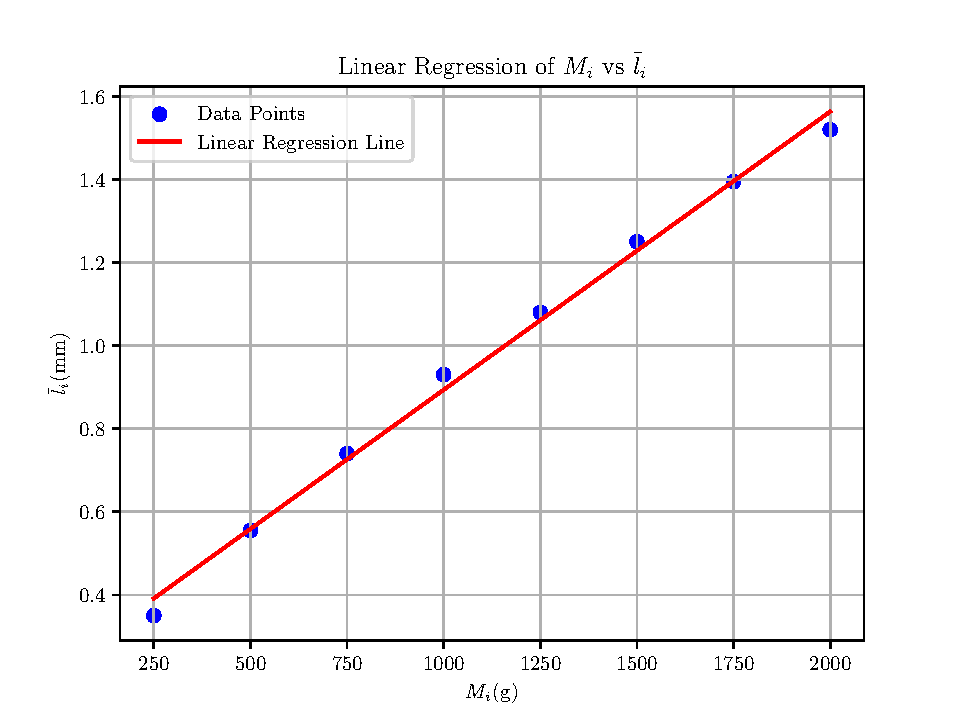
\includegraphics[width=0.8\textwidth]{plot1.pdf}
    \caption{作图法处理杨氏模量}
\end{figure}

\subsection{讨论}
\subsubsection{实验中遇到的问题}
在实验操作中，一定要注意加减砝码时得轻拿轻放，否则就需要等待很长一段时间使得砝码盘停止振荡。

在实验数据的处理过程中，我发现我最后得到的测量数据和参考数据的相对误差较大，这可能是由于以下几点原因造成的：
\begin{enumerate}
    \item $L$难以测量精确，这是因为实验中使用的卷尺在测量钼丝长度时很难确定是否将卷尺的起始位置对准了钼丝的起始位置，同时在测量时也很难保证和钼丝平行，这样就会导致测量结果的误差。
    \item 砝码质量偏小。实验过程中发现砝码有部分生锈，可能导致砝码的实际重量比标示的重量更大，导致测量误差。
    \item 试验台未调整水平。实验过程中我使用的那台实验台没有水平计，所以无法保证实验台的水平，这样就会导致实验过程中的误差。
\end{enumerate}

\subsubsection{可能的改进方法}
\begin{enumerate}
    \item 使用更精确的测量仪器。可以使用更精确的测量仪器来测量钼丝的长度和直径(比如说直接拿一根线来对准钼丝两端，最后再用米尺测量对应得线得长度)，这样可以减小测量误差。
    \item 使用更精确的砝码，并尽可能用专门的夹具来夹住砝码，而不是直接用手拿，这样可以缓解砝码的生锈问题。
    \item 保证实验台水平。在实验开始前应该先调整实验台使得水平仪显示水平，这样可以减小实验过程中的误差。
\end{enumerate}

\subsection{思考题}
\subsubsection{杨氏模量测量数据 $N$ 若不用逐差法而用作图法，如何处理?}
变形杨氏模量公式可得
\[
l_i = \frac{L}{Y}\left(\frac{m_i g}{S}\right) + l_0 - l = km_i + b,
\]
其中
\[
k = \frac{4gL}{\pi d^2 Y},
\]
于是
\[
Y = \frac{4gL}{\pi d^2 k}.
\]
以$m_i$为横坐标，以$l_i$为纵坐标，建立直角坐标系，将测量数据在坐标系中标出，画出一条直线，让散点尽量均匀地分布在直线的两侧，再在直线上选取较远的两个点，求出直线的斜率，代入公式即可求得杨氏模量$Y$。

\subsubsection{两根材料相同但粗细不同的金属丝，它们的杨氏模量相同吗？为什么？}
相同，因为杨氏模量是材料本身的性质，与材料的长度大小、粗细程度等无关。

\subsubsection{本实验使用了哪些测量长度的量具？选择它们的依据是什么？它们的仪器误差各是多少？}
\begin{enumerate}
    \item 本实验使用了卷尺、螺旋测微器和CCD杨氏模量测量仪。
    \item 选择依据如下：
    \begin{itemize}
        \item 之所以选择卷尺测量钼丝的长度，是因为钼丝的长度较长，卷尺的量程较大，所以采用卷尺来测量钼丝长度；
        \item 之所以选择螺旋测微器测量钼丝的直径，是因为钼丝的直径较小，对测量的精度要求较高，而螺旋测微器在测量微小长度时具有较高精度；
        \item 之所以选择CCD杨氏模量测量仪测量钼丝的伸长量，是因为钼丝的伸长量极小，且不适合运用螺旋测微器测量，所以采用选择CCD杨氏模量测量仪测量，其最小分度值为0.05mm符合要求。
    \end{itemize}

    \item 卷尺的允差为2 mm，螺旋测微器的允差为0.005 mm，CCD杨氏模量测量仪的允差为0.001 mm。
\end{enumerate}

\subsubsection{在 CCD 法测定金属丝杨氏模量实验中，为什么起始时要加一定数量的底码？}
底码的作用是把钼丝拉直，由此减小测量误差。底码也可以稳定分划板，方便读数。

\subsubsection{加砝码后标示横线在屏幕上可能上下颤动不停，不能够完全稳定时，如何判定正确读数？}
可以用手轻轻拖住砝码托盘，等其稳定后放开进行测量。
\section{使用霍尔传感器测杨氏模量}
\subsection{实验目的}
\begin{enumerate}
    \item 熟悉霍尔位置传感器的特性，完成样品的测量和对霍尔位置传感器定标，理解传感器特定曲线对测量的意义；
    \item 学会读数望远镜、读数显微镜的调节；
    \item 学习用逐差法、作图法和最小二乘法处理数据；
    \item 学会计算各物理量的不确定度，并用不确定度正确表达实验结果。
\end{enumerate}

\subsection{实验仪器}
\subsubsection{杭州大华DHY-A霍尔位置传感器法杨氏模量测定仪}
\begin{itemize}
    \item 读数显微镜 型号 JC-10 型
          目镜放大率 10 倍
          目镜测微鼓轮最小分度值 0.01mm
          物镜放大率 2 倍
          测量范围 0～6mm
          鼓轮实际读数最小分辨率 0.01/2=0.005mm
    \item 电子称传感器加力系统：0-199.9g 连续可调，三位半数显。
    \item 霍尔电压表：量程 1：0～199.9mV，分辨率 0.1mV；
                       量程 2：0～1.999V，分辨率 1mV。
    \item 霍尔位置传感器：灵敏度大于 250mV/mm，线性范围 0～2mm。
\end{itemize}
\subsubsection{长度测量仪器}
\begin{itemize}
    \item 钢板尺（量程300mm，分度值1mm）
    \item 游标卡尺（量程125mm，分度值0.02mm）
    \item 螺旋测微器（量程25mm，分度值0.01mm）
\end{itemize}

\subsection{实验原理}
霍尔元件在稳定电场中，若$\frac{dB}{dZ}$为常数，则$\Delta U$与$\Delta Z$成正比，在位移量较小的时候，霍尔电势差与位移量有着较好的线性一一对应关系，在横梁弯曲的情况下，杨氏模量$Y$可以用下式表示：
\begin{equation}
    Y = \frac{d^3 Mg}{4a^3 b\Delta Z}
\end{equation}

\subsection{实验内容}
\begin{enumerate}
    \item 按照实验装置示意图安装实验仪器。
    \item 调节使得霍尔位置传感器探测元件处在磁铁中间的位置。
    \item 移动磁铁将霍尔电压调到一个微小值，然后通过霍尔位置传感器上的调零旋钮将电压调零。
    \item 调节读数显微镜目镜，使得眼睛能看到十字线、分划板刻度线和数字清晰。调整前后距离看到基线。再转动读数显微镜上的读数鼓轮使得铜刀口上的基线和读数显微镜内十字刻度线吻合，记下初始读数值。
\end{enumerate}

\subsection{实验数据}
\subsubsection{样品一: 黄铜}
\begin{itemize}
    \item 横梁的几何尺寸
        \begin{table}[H]
        \centering
        \begin{tabular}{|c|c|c|c|c|c|c|c|} 
        \hline
        测量次数   & 1     & 2     & 3     & 4     & 5     & 6     & 平均值    \\ 
        \hline
        长度$d$/mm & 299.7 & 299.8 & 299.7 & 299.9 & 300.0 & 299.8 & 299.8  \\ 
        \hline
        宽度$b$/mm & 23.10 & 24.00 & 23.20 & 23.24 & 23.10 & 23.80 & 23.41  \\ 
        \hline
        厚度$a$/mm & 1.045 & 1.046 & 1.042 & 1.040 & 1.046 & 1.040 & 1.043  \\
        \hline
        \end{tabular}
        \caption{黄铜横梁的几何尺寸}
        \end{table}
    \item 读数显微镜示数
    显微镜初始读数$Z_0 = 2.920$mm
\end{itemize}
\begin{table}[H]
\centering
\begin{tabular}{|c|c|c|c|c|c|c|c|c|c|} 
\hline
序号                                & 1      & 2      & 3      & 4      & 5     & 6     & 7     & 8     & 平均值     \\ 
\hline
$M_i$/g                        & 20.1   & 39.7  & 59.7   & 80.0     & 99.9  & 120.0   & 139.8 & 159.8 & 89.9   \\ 
\hline
$Z_i$/mm                       & 2.565  & 2.341  & 2.145  & 1.876  & 1.632 & 1.335 & 1.081 & 0.741 & 1.715   \\ 
\hline
$U_i$/mV                       & 34     & 75     & 110    & 148    & 184   & 221   & 256   & 289   & 165     \\ 
\hline
$\Delta Z_i$/mm                & -0.933 & -1.006 & -1.064 & -1.135 &       &       &       &       & -1.035  \\ 
\hline
$\Delta U_i$/mV                & 150    & 146    & 146    & 141    &       &       &       &       & 146     \\ 
\hline
$U_i^2$ /mV$^2$ & 1156   & 5625   & 12100  & 21904  & 33856 & 48841 & 65536 & 83521 & 34067   \\ 
\hline
 $Z_i^2$ /mm$^2$   & 6.579  & 5.480  & 4.601  & 3.519  & 2.663 & 1.782 & 1.169 & 0.549 & 3.293   \\ 
\hline
$Z_iU_i$ / (mm $\cdot$ mV)  & 87     & 176    & 236    & 278    & 300   & 295   & 277   & 214   & 233     \\ 
\hline
\end{tabular}
\caption{黄铜读数显微镜示数}
\end{table}

\subsubsection{样品二: 铸铁}
\begin{itemize}
    \item 横梁的几何尺寸
        \begin{table}[H]
        \centering
        \begin{tabular}{|c|c|c|c|c|c|c|c|} 
        \hline
        测量次数   & 1     & 2     & 3     & 4     & 5     & 6     & 平均值    \\ 
        \hline
        长度d/mm & 300.1 & 299.8 & 300.2 & 299.6 & 299.6 & 299.6 & 299.8  \\ 
        \hline
        宽度b/mm & 23.40 & 23.10 & 23.00 & 23.80 & 23.40 & 23.40 & 23.35  \\ 
        \hline
        厚度a/mm & 1.047 & 1.048 & 1.040  & 1.047 & 1.042 & 1.044 & 1.045  \\
        \hline
        \end{tabular}
        \caption{铸铁横梁的几何尺寸}
        \end{table}
    \item 读数显微镜示数
    显微镜初始读数$Z_0 = 4.069$mm
\end{itemize}
\begin{table}[H]
\centering
\begin{tabular}{|c|c|c|c|c|c|c|c|c|c|} 
\hline
序号                                & 1      & 2      & 3      & 4      & 5     & 6     & 7     & 8     & 平均值     \\ 
\hline
$M_i$/g          & 19.9   & 40.1   & 59.7   & 80.4   & 100.0  & 120.2  & 139.9  & 160.2  & 90.1    \\ 
\hline
$Z_i$/mm         & 3.895  & 3.802  & 3.710  & 3.581  & 3.439  & 3.318  & 3.171  & 3.304  & 3.528   \\ 
\hline
$U_i$/mV         & 19     & 38     & 57     & 77     & 96     & 114    & 131    & 147    & 85      \\ 
\hline
$\Delta Z_i$/mm   & -0.456 & -0.484 & -0.539 & -0.277 &        &        &        &        & -0.439  \\ 
\hline
$\Delta U_i$/mV   & 77     & 76     & 74     & 70     &        &        &        &        & 74      \\ 
\hline
$U_i^2$ /mV$^2$       & 361    & 1444   & 3249   & 5929   & 9216   & 12996  & 17161  & 21609  & 8996    \\ 
\hline
 $Z_i^2$ /mm$^2$       & 15.171 & 14.455 & 13.764 & 12.824 & 11.827 & 11.009 & 10.055 & 10.916 & 12.503  \\ 
\hline
$Z_iU_i$ / (mm $\cdot$ mV) & 74     & 144    & 211    & 276    & 330    & 378    & 415    & 486    & 289     \\
\hline
\end{tabular}
\caption{铸铁读数显微镜示数}
\end{table}
\subsection{数据处理}
\subsubsection{黄铜长度}
利用钢板尺对黄铜的长度\( d \)进行单次测量，测量结果为\( d = 299.8 \, \text{mm} \)。所以有A类不确定度
\[
u_A (d) = \sqrt{\frac{\sum_{i=1}^{6} (d_i - \bar{d})^2}{6(6-1)}} = \sqrt{\frac{0.1^2 + 0.0^2 + 0.1^2 + 0.1^2 + 0.2^2 + 0.0^2}{30}} = \sqrt{\dfrac{7}{3000}} \, \text{mm}
\]
由于钢板尺的允差\( e = 0.12 \, \text{mm} \)，所以B类不确定度为
\[ u_B (L) = \frac{e}{\sqrt{3}} = \frac{0.12}{\sqrt{3}} \, \text{mm}. \]
所以测量黄铜长度的不确定度\( u(d) \)为
\[ u(d) = \sqrt{u_A (d)^2 + u_B (d)^2} = \sqrt{\left(\frac{0.12}{\sqrt{3}}\right)^2 + \frac{7}{3000}} = 0.1 \, \text{mm}. \]
其相对不确定度为
\[ \frac{u(d)}{d} = \frac{0.1}{299.8} \times 100\% = 0.03\%. \]
黄铜的长度为
\[ d = (299.8 \pm 0.1) \, \text{mm}. \]

\subsubsection{铸铁长度}
利用钢板尺对铸铁的长度\( d \)进行单次测量，测量结果为\( d = 299.8 \, \text{mm} \)。所以有A类不确定度
\[
u_A (d) = \sqrt{\frac{\sum_{i=1}^{6} (d_i - \bar{d})^2}{6(6-1)}} = \sqrt{\frac{0.3^2 + 0.0^2 + 0.4^2 + 0.2^2 + 0.2^2 + 0.2^2}{30}} = \sqrt{\dfrac{37}{3000}} \, \text{mm}
\]
由于钢板尺的允差\( e = 0.12 \, \text{mm} \)，所以B类不确定度为
\[ u_B (L) = \frac{e}{\sqrt{3}} = \frac{0.12}{\sqrt{3}} \, \text{mm}. \]
所以测量铸铁长度的不确定度\( u(d) \)为
\[ u(d) = \sqrt{u_A (d)^2 + u_B (d)^2} = \sqrt{\left(\frac{0.12}{\sqrt{3}}\right)^2 + \frac{37}{3000}} = 0.1 \, \text{mm}. \]
其相对不确定度为
\[ \frac{u(d)}{d} = \frac{0.1}{299.8} \times 100\% = 0.03\%. \]
铸铁的长度为
\[ d = (299.8 \pm 0.1) \, \text{mm}. \]

\subsubsection{黄铜宽度}
利用游标卡尺对黄铜的宽度 \( b \) 进行单次测量，测量结果为 \( b = 23.41 \, \text{mm} \)。由于测量次数为6，所以A类不确定度
\[ u_A (b) = \sqrt{\frac{\sum_{i=1}^{6}(b_i - \bar{b})^2}{6(6-1)}} = \sqrt{\frac{0.31^2 + 0.59^2 + 0.21^2 + 0.17^2 + 0.31^2 + 0.39^2}{30}} = \sqrt{0.01391} \, \text{mm} \]
由于游标卡尺的允差 \( e = 0.02 \, \text{mm} \)，所以B类不确定度为
\[ u_B (b) = \frac{e}{\sqrt{3}} = \frac{0.02}{\sqrt{3}} \, \text{mm}. \]
所以测量黄铜宽度的不确定度 \( u(b) \) 为
\[ u(b) = \sqrt{u_A (b)^2 + u_B (b)^2} = \sqrt{\frac{0.02^2}{3} + 0.01391} = 0.12 \, \text{mm}. \]
其相对不确定度为
\[ \frac{u(b)}{b} = \frac{0.12}{23.41} \times 100\% = 0.51\%. \]
黄铜的宽度为
\[ b = (23.41 \pm 0.12) \, \text{mm}. \]

\subsubsection{铸铁宽度}
利用游标卡尺对铸铁的宽度 \( b \) 进行单次测量，测量结果为 \( b = 23.35 \, \text{mm} \)。由于测量次数为6，所以A类不确定度
\[ u_A (b) = \sqrt{\frac{\sum_{i=1}^{6}(b_i - \bar{b})^2}{6(6-1)}} = \sqrt{\frac{0.05^2 + 0.25^2 + 0.35^2 + 0.45^2 + 0.05^2 + 0.05^2}{30}} = \sqrt{0.01317} \, \text{mm} \]
由于游标卡尺的允差 \( e = 0.02 \, \text{mm} \)，所以B类不确定度为
\[ u_B (b) = \frac{e}{\sqrt{3}} = \frac{0.02}{\sqrt{3}} \, \text{mm}. \]
所以测量铸铁宽度的不确定度 \( u(b) \) 为
\[ u(b) = \sqrt{u_A (b)^2 + u_B (b)^2} = \sqrt{\frac{0.02^2}{3} + 0.01317} = 0.12 \, \text{mm}. \]
其相对不确定度为
\[ \frac{u(b)}{b} = \frac{0.12}{23.35} \times 100\% = 0.51\%. \]
铸铁的宽度为
\[ b = (23.35 \pm 0.12) \, \text{mm}. \]

\subsubsection{黄铜厚度}
利用螺旋测微器对黄铜的厚度 \( a \) 进行单次测量，测量结果为 \( a = 1.043 \, \text{mm} \)。由于测量次数为6，所以A类不确定度
\[ u_A (a) = \sqrt{\frac{\sum_{i=1}^{6}(a_i - \bar{a})^2}{6(6-1)}} = \sqrt{\frac{0.002^2 + 0.003^2 + 0.001^2 + 0.003^2 + 0.003^2 + 0.003^2}{30}} = \sqrt{1.367 \times 10^{-6}} \, \text{mm} \]
由于螺旋测微器的允差 \( e = 0.005 \, \text{mm} \)，所以B类不确定度为
\[ u_B (a) = \frac{e}{\sqrt{3}} = \frac{0.005}{\sqrt{3}} \, \text{mm}. \]
所以测量黄铜厚度的不确定度 \( u(a) \) 为
\[ u(a) = \sqrt{u_A (a)^2 + u_B (a)^2} = \sqrt{\frac{0.005^2}{3} + 1.367 \times 10^{-6}} = 0.003 \, \text{mm}. \]
其相对不确定度为
\[ \frac{u(a)}{a} = \frac{0.003}{1.043} \times 100\% = 0.29\%. \]
黄铜的厚度为
\[ a = (1.043 \pm 0.003) \, \text{mm}. \]

\subsubsection{铸铁厚度}
利用螺旋测微器对铸铁的厚度 \( a \) 进行单次测量，测量结果为 \( a = 1.045 \, \text{mm} \)。由于测量次数为6，所以A类不确定度
\[ u_A (a) = \sqrt{\frac{\sum_{i=1}^{6}(a_i - \bar{a})^2}{6(6-1)}} = \sqrt{\frac{0.002^2 + 0.003^2 + 0.005^2 + 0.002^2 + 0.003^2 + 0.001^2}{30}} = \sqrt{1.733 \times 10^{-6}} \, \text{mm} \]
由于螺旋测微器的允差 \( e = 0.005 \, \text{mm} \)，所以B类不确定度为
\[ u_B (a) = \frac{e}{\sqrt{3}} = \frac{0.005}{\sqrt{3}} \, \text{mm}. \]
所以测量铸铁厚度的不确定度 \( u(a) \) 为
\[ u(a) = \sqrt{u_A (a)^2 + u_B (a)^2} = \sqrt{\frac{0.005^2}{3} + 1.733 \times 10^{-6}} = 0.003 \, \text{mm}. \]
其相对不确定度为
\[ \frac{u(a)}{a} = \frac{0.003}{1.045} \times 100\% = 0.29\%. \]
铸铁的厚度为
\[ a = (1.045 \pm 0.003) \, \text{mm}. \]

\subsubsection{黄铜弯曲位移}
通过显微镜观察得到$\Delta Z$，其A类不确定度为
\[ u_A (\Delta Z) = \sqrt{\frac{\sum_{i=1}^{4}(\Delta Z_i - \overline{\Delta Z})^2}{4(4-1)}} = \sqrt{\frac{0.102^2 + 0.029^2 + 0.029^2 + 0.1^2}{12}} = \sqrt{1.84 \times 10^{-3}} \text{mm} \]
由于电子刻度线的允差$e=0.002$ mm，所以B类不确定度为
\[ u_B (L) = \frac{e}{\sqrt{3}} = \frac{0.002}{\sqrt{3}} \text{mm}. \]
所以测量弯曲位移的不确定度$u(\Delta Z)$为
\[ u(\Delta Z) = \sqrt{u_A (\Delta Z)^2 + u_B (\Delta Z)^2} = \sqrt{\frac{0.002^2}{3} + 1.84 \times 10^{-3}} = 0.043 \text{mm}. \]
其相对不确定度为
\[ \frac{u(\Delta Z)}{\Delta Z} = \frac{0.043}{1.035} \times 100\% = 4.14\%. \]
弯曲位移为
\[ \Delta Z = (1.035 \pm 0.043) \text{mm}. \]

\subsubsection{铸铁弯曲位移}
通过显微镜观察得到$\Delta Z$，其A类不确定度为
\[ u_A (\Delta Z) = \sqrt{\frac{\sum_{i=1}^{4}(\Delta Z_i - \overline{\Delta Z})^2}{4(4-1)}} = \sqrt{\frac{0.017^2 + 0.045^2 + 0.1^2 + 0.162^2}{12}} = \sqrt{3.21 \times 10^{-3}} \text{mm} \]
由于电子刻度线的允差$e=0.002$ mm，所以B类不确定度为
\[ u_B (L) = \frac{e}{\sqrt{3}} = \frac{0.002}{\sqrt{3}} \text{mm}. \]
所以测量弯曲位移的不确定度$u(\Delta Z)$为
\[ u(\Delta Z) = \sqrt{u_A (\Delta Z)^2 + u_B (\Delta Z)^2} = \sqrt{\frac{0.002^2}{3} + 3.21 \times 10^{-3}} = 0.057 \text{mm}. \]
其相对不确定度为
\[ \frac{u(\Delta Z)}{\Delta Z} = \frac{0.057}{0.439} \times 100\% = 13.0\%. \]
弯曲位移为
\[ \Delta Z = (0.439 \pm 0.057) \text{mm}. \]

\subsubsection{黄铜杨氏模量}
根据已知数据和公式计算可得：
\[ Y=\frac{(299.8)^3 \times 69.9 \times 9.81}{4 \times (1.043)^3 \times 23.41 \times 1.035 \times 10^{-3}} = 16.80 \times 10^{10} \, \text{N}\cdot\text{m}^{-2}. \]
由于黄铜杨氏模量的参考值为 \( Y_0 = 10.55 \times 10^{10} \, \text{N}\cdot\text{m}^{-2} \)，因此相对误差为
\[ E_r = \left| \frac{Y - Y_0}{Y_0} \right| \times 100\% = \left| \frac{10.55 - 16.80}{10.55} \right| \times 100\% = 59.2\%. \]

\subsubsection{铸铁杨氏模量}
根据已知数据和公式计算可得：
\[ Y=\frac{(299.8)^3 \times 69.1 \times 9.81}{4 \times (1.045)^3 \times 23.35 \times 0.439 \times 10^{-3}} = 39.03 \times 10^{10} \, \text{N}\cdot\text{m}^{-2}. \]
由于铸铁杨氏模量的参考值为 \( Y_0 = 18.15 \times 10^{10} \, \text{N}\cdot\text{m}^{-2} \)，因此相对误差为
\[ E_r = \left| \frac{Y - Y_0}{Y_0} \right| \times 100\% = \left| \frac{18.15 - 39.03}{18.15} \right| \times 100\% = 115.0\%. \]

\subsubsection{最小二乘法拟合灵敏系数}
分别对黄铜和铸铁的数据作图，并进行最小二乘法拟合，得到如下结果：

\begin{figure}[H]
    \centering
    \begin{minipage}[t]{0.45\textwidth}
        \centering
        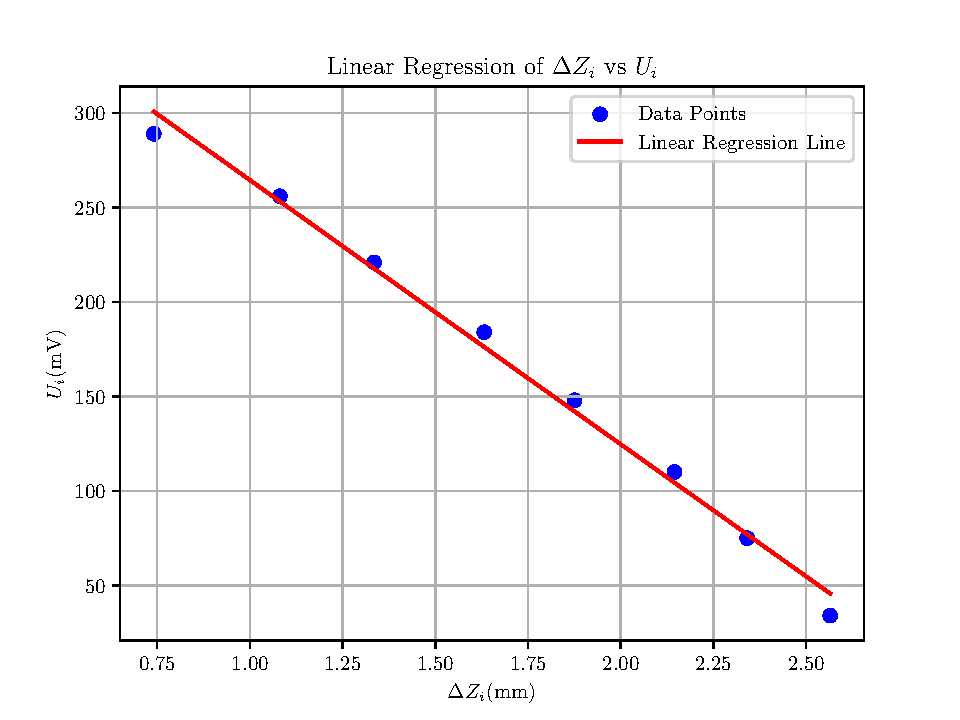
\includegraphics[width=0.95\textwidth]{plot2.pdf}
        \caption{黄铜数据拟合}
    \end{minipage}%
    \begin{minipage}[t]{0.45\textwidth}
        \centering
        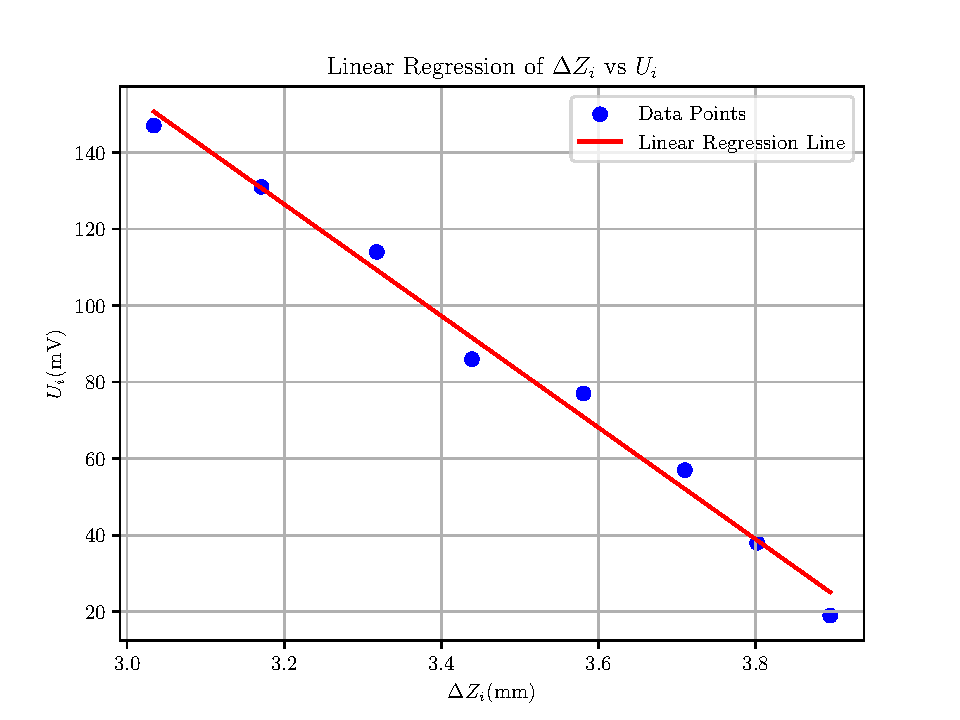
\includegraphics[width=0.95\textwidth]{plot3.pdf}
        \caption{铸铁数据拟合}
    \end{minipage}
\end{figure}
拟合直线对应的灵敏系数分别为
\[ k_{\text{黄铜}} = 140 \, \text{mV/mm} \]
\[ k_{\text{铸铁}} = 146 \, \text{mV/mm} \]

\subsection{讨论}
\begin{enumerate}
    \item 实验中需要通过调整旋钮来给加力机构加力，在旋转的过程中必须十分小心，一旦超过了读数范围就无法回头，只能重新开始。
    \item 本次实验中我测量的杨氏模量的误差比前一次实验中要大得多，这可能是因为刚开始测量时加力得绳丝没有完全拉直，以及横梁弯曲的方向并不是严格的竖直向下导致的
    \item 读数显微镜的读数较为困难，横梁上的划线比较难以看清，且显微镜结构对近视的人不太友好
\end{enumerate}

\subsection{思考题}
\subsubsection{弯曲法测杨氏模量实验，主要测量误差有哪些? 请估算各因素的不确定度}
\begin{enumerate}
    \item 样品厚度的误差, $u(a) \approx 0.005$mm
    \item 样品长度的误差, $u(d) \approx 0.1$mm
    \item 样品宽度的误差, $u(b) \approx 0.02$mm
    \item 弯曲位移的误差, $u(\Delta Z) \approx 0.0026$mm
\end{enumerate}
\subsubsection{用霍尔位置传感器法测位移有什么优点?}
霍尔位置传感器法测位移的优点有：
\begin{enumerate}
    \item 测量精度高，可以达到亚毫米级别
    \item 非接触式测量，能够减小误差
    \item 测量速度快，可以达到几百次每秒
    \item 具有良好的线性
\end{enumerate}
\subsubsection{请自行分析实验过程中和数据分析中遇到的问题，找到处理方法}
比如说讨论中提到的显微镜的读数较为困难的问题，可以通过导出数据后用计算机进行处理，减小人为误差。

\section{动态悬挂法测杨氏模量}

\subsection{实验目的}
\begin{enumerate}
    \item 学会用动态悬挂法测量材料的杨氏模量；
    \item 学习用外延法测量，处理实验数据；
    \item 了解换能器的功能，熟悉测试仪器及示波器的使用；
    \item 培养学生综合运用知识和使用常用实验仪器的能力。
\end{enumerate}

\subsection{实验仪器}
DHY-2A 动态杨氏模量测试台、DH0803 振动力学通用信号源，通用示波器、测试棒（铜、不锈钢）、悬线、专用连接导线、天平、游标卡尺（量程125mm，分度值0.02mm），螺旋测微器（量程25mm，分度值0.01mm）等。

\subsection{实验原理}
当金属棒达到共振时，根据棒的横振动方程和频率公式，可以求出在基频下共振时，有公式：
\[ Y = 1.6067 \frac{L^3 m f_1^2}{d^4} \]
测量出$L$, $m$, $d$后，近似找到$f_1$，即算出$Y$值大小。

\subsection{实验内容}
\begin{enumerate}
    \item 测量黄铜棒的长度$L$，直径$d$，质量$m$；
    \item 将黄铜棒悬挂在水平悬线上；
    \item 一边改变输入信号频率，一边观察示波器，当波峰达到最大时，记录此时的频率，即共振频率
    \item 更换悬挂点位置进行多次实验
\end{enumerate}

\subsection{实验数据}
\begin{itemize}
    \item 黄铜棒的长度$L = 180.2$mm，直径$d = 5.961$mm，质量$m = 42.18$g；
    \item 悬挂点位置和共振频率关系如下：
        \begin{table}[H]
        \centering
        \begin{tabular}{|c|c|c|c|c|c|c|c|c|} 
        \hline
        序号        & 1       & 2       & 3       & 4       & 5       & 6       & 7       & 8        \\ 
        \hline
        悬挂点位置$x$/mm & 20      & 25      & 30      & 35      & 45      & 50      & 55      & 60       \\ 
        \hline
        $x/L$       & 0.111   & 0.139   & 0.166   & 0.194   & 0.250   & 0.277   & 0.305   & 0.333    \\ 
        \hline
        共振频率$f_1$/Hz & 590.620 & 588.321 & 586.620 & 585.521 & 585.321 & 586.121 & 587.221 & 588.521  \\
        \hline
        \end{tabular}
        \caption{悬挂点位置和共振频率关系}
        \end{table}
\end{itemize}
\subsection{数据处理}
\subsubsection{黄铜棒共振频率}
根据表8的数据，作图并作二次多项式拟合，得到如下结果：
\begin{figure}[H]
    \centering
    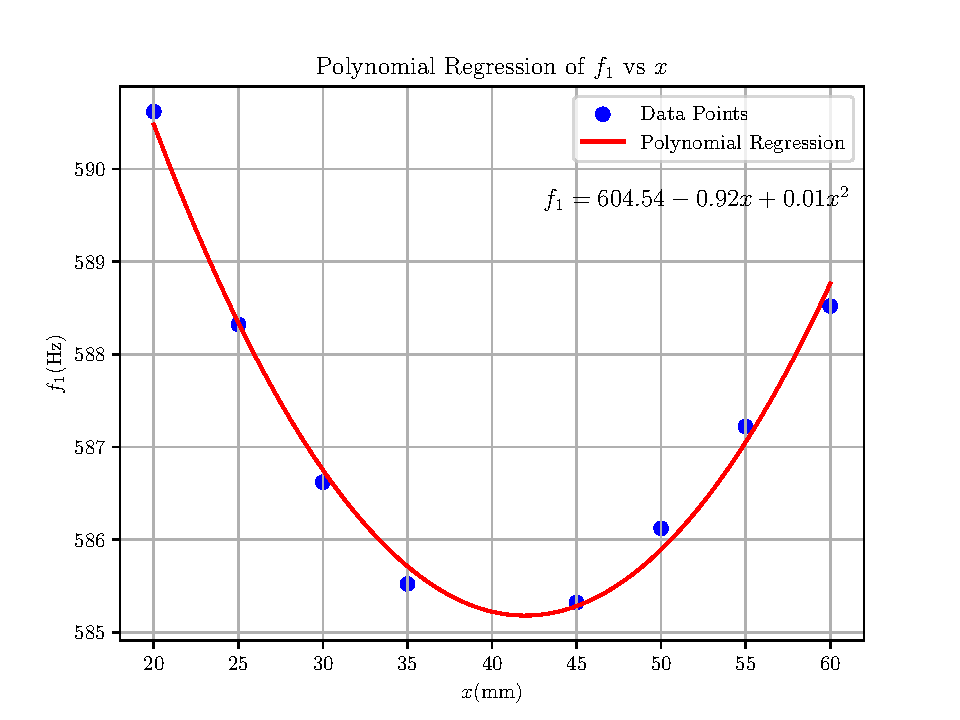
\includegraphics[width=0.6\textwidth]{plot4.pdf}
    \caption{黄铜棒共振频率}
\end{figure}
其中拟合方程为
\[ \hat{f_1} = 0.01x^2 - 0.92x + 604.54 \]
且最低点在$(41.94\text{mm}, 585.18\text{Hz})$处取到
\subsubsection{黄铜杨氏模量}
根据已知数据和公式计算可得：
\[ Y = 1.6067 \frac{L^3 m f_1^2}{d^4} = 1.6067 \frac{(180.2)^3 \times 42.18 \times (585.18)^2}{(5.961)^4} = 1.08 \times 10^{11} \, \text{N}\cdot\text{m}^{-2}. \]
这个结果在黄铜棒的杨氏模量的参考值范围$Y' = 0.8 \sim 1.10 \times 10^{11} \, \text{N}\cdot\text{m}^{-2}$内，所以可以认为实验结果是正确的。

\subsection{讨论}
由于本次实验中的原始数据表格中没有要求记录多次测量样品参数的结果，所以这里不进行不确定度的计算。就结果而言，实验结果与参考值较为接近，实验结果较为精确

在观察示波器的过程中，可能会出现“假共振”的情况，即示波器显示的波形并不是真正的共振波形。这时候我们可以以通过给棒的$40$mm处施加一个力，如果波形不再稳定，那么就是假共振

在悬挂棒的过程中，需要注意悬挂线要和棒垂直，以减小误差
\subsection{思考题}
\subsubsection{外延测量法有什么特点？使用时应注意什么问题？}
即根据已知范围内的数据来推测未知范围内数据的规律，所以预测的数据不一定准确，使用时应该注意结果与客观规律的契合，减少主观对于客观规律的影响
\subsubsection{物体的固有频率和共振频率有什么不同？它们之间有何关系}
固有频率是物体自身振动时的频率，共振频率是物体受迫振动时振幅最大的频率，两者是不同的概念，它们的关系是
\[ f_\text{固有} = f_\text{共振} \sqrt{1 + \dfrac{1}{4Q^2}} \]
% 内嵌pdf
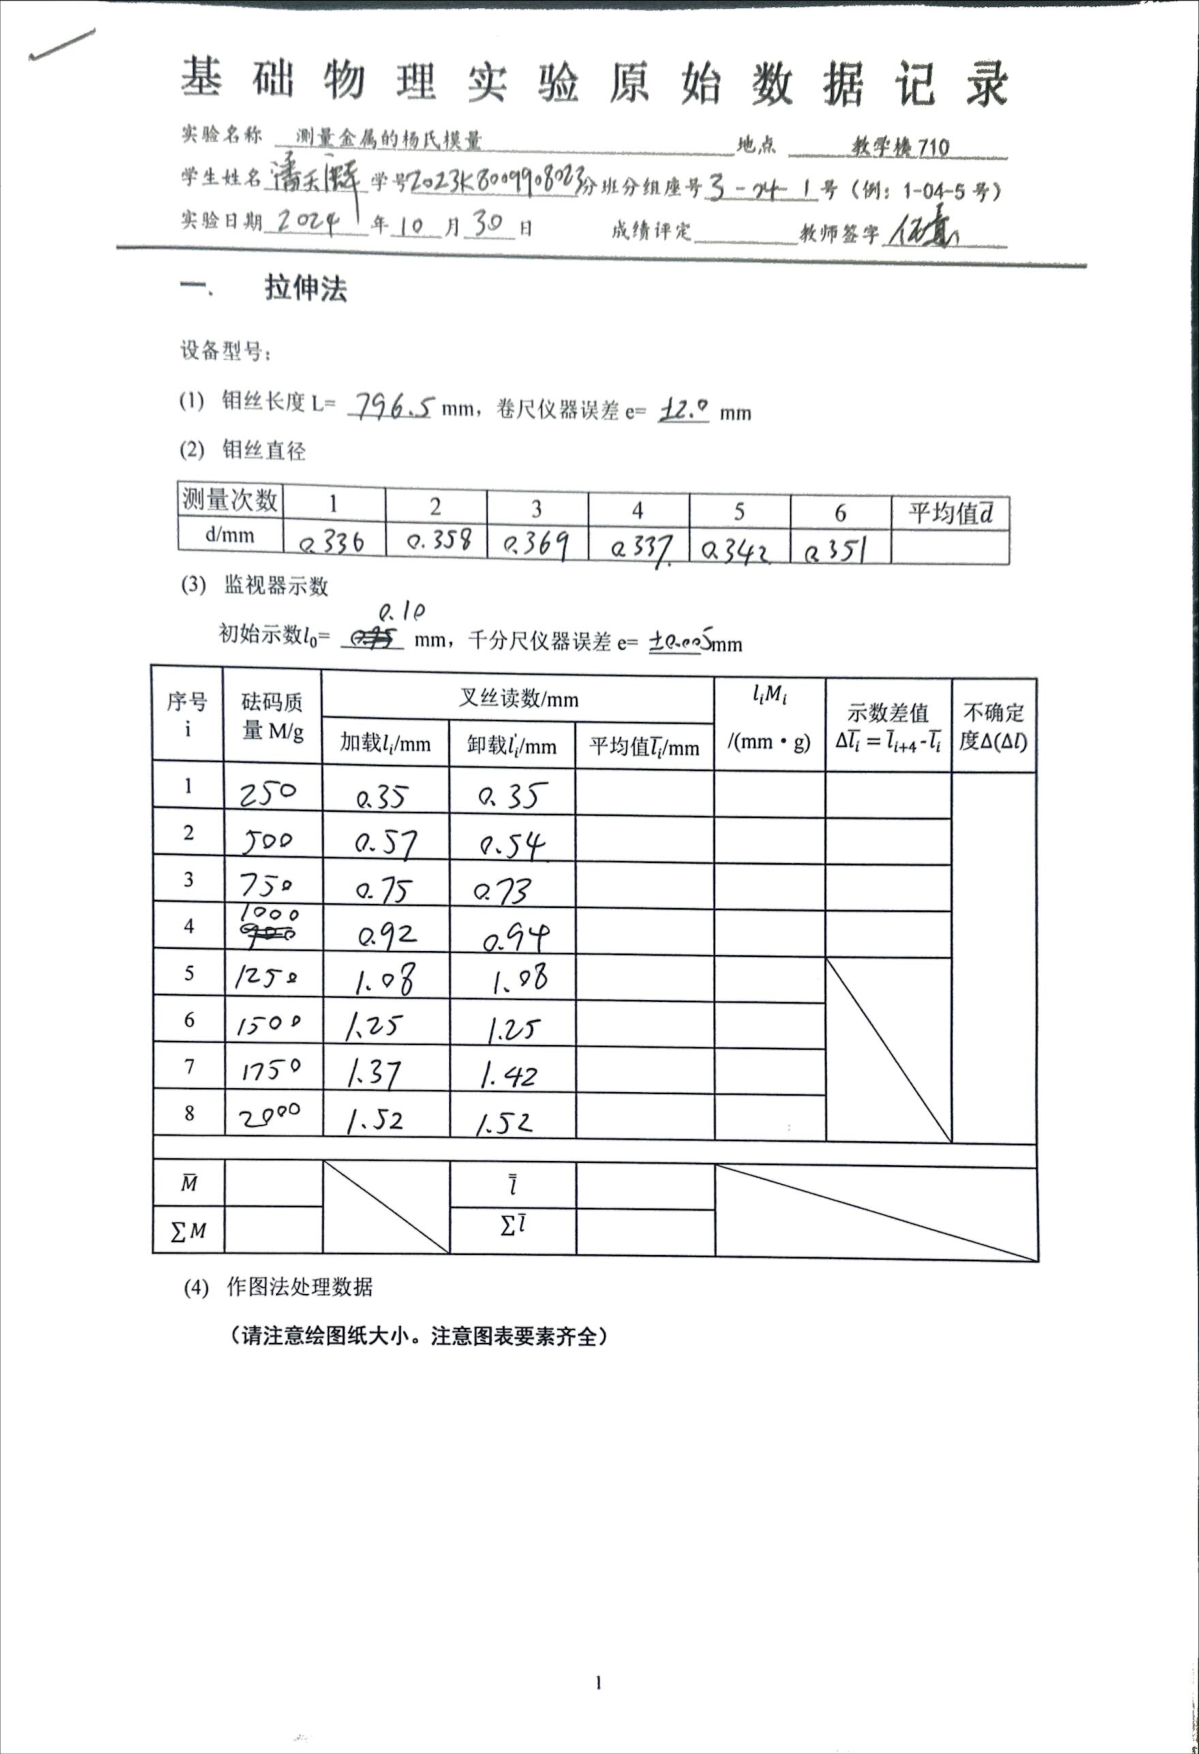
\includepdf[pages=-]{原始数据.pdf}
\end{document}
